\documentclass[spec, och, labwork]{shiza}
% параметр - тип обучения - одно из значений:
%    spec     - специальность
%    bachelor - бакалавриат (по умолчанию)
%    master   - магистратура
% параметр - форма обучения - одно из значений:
%    och   - очное (по умолчанию)
%    zaoch - заочное
% параметр - тип работы - одно из значений:
%    referat    - реферат
%    coursework - курсовая работа (по умолчанию)
%    diploma    - дипломная работа
%    pract      - отчет по практике
% параметр - включение шрифта
%    times    - включение шрифта Times New Roman (если установлен)
%               по умолчанию выключен
\usepackage{subfigure}
\usepackage{tikz,pgfplots}
\pgfplotsset{compat=1.5}
\usepackage{float}

%\usepackage{titlesec}
\setcounter{secnumdepth}{4}
%\titleformat{\paragraph}
%{\normalfont\normalsize}{\theparagraph}{1em}{}
%\titlespacing*{\paragraph}
%{35.5pt}{3.25ex plus 1ex minus .2ex}{1.5ex plus .2ex}

\titleformat{\paragraph}[block]
{\hspace{1.25cm}\normalfont}
{\theparagraph}{1ex}{}
\titlespacing{\paragraph}
{0cm}{2ex plus 1ex minus .2ex}{.4ex plus.2ex}

% --------------------------------------------------------------------------%


\usepackage[T2A]{fontenc}
\usepackage[utf8]{inputenc}
\usepackage{graphicx}
\graphicspath{ {./images/} }
\usepackage{tempora}

\usepackage[sort,compress]{cite}
\usepackage{amsmath}
\usepackage{amssymb}
\usepackage{amsthm}
\usepackage{fancyvrb}
\usepackage{listings}
\usepackage{listingsutf8}
\usepackage{longtable}
\usepackage{array}
\usepackage[english,russian]{babel}

% \usepackage[colorlinks=true]{hyperref}
\usepackage{url}

\usepackage{underscore}
\usepackage{setspace}
\usepackage{indentfirst} 
\usepackage{mathtools}
\usepackage{amsfonts}
\usepackage{enumitem}
\usepackage{tikz}
\usepackage{minted}

\newcommand{\eqdef}{\stackrel {\rm def}{=}}
\newcommand{\specialcell}[2][c]{%
\begin{tabular}[#1]{@{}c@{}}#2\end{tabular}}

\renewcommand\theFancyVerbLine{\small\arabic{FancyVerbLine}}

\newtheorem{lem}{Лемма}

\begin{document}

% Кафедра (в родительном падеже)
\chair{}

% Тема работы
\title{Классификация бинарных отношений и системы замыканий}

% Курс
\course{3}

% Группа
\group{331}

% Факультет (в родительном падеже) (по умолчанию "факультета КНиИТ")
\department{факультета КНиИТ}

% Специальность/направление код - наименование
%\napravlenie{09.03.04 "--- Программная инженерия}
%\napravlenie{010500 "--- Математическое обеспечение и администрирование информационных систем}
%\napravlenie{230100 "--- Информатика и вычислительная техника}
%\napravlenie{231000 "--- Программная инженерия}
\napravlenie{100501 "--- Компьютерная безопасность}

% Для студентки. Для работы студента следующая команда не нужна.
% \studenttitle{Студентки}

% Фамилия, имя, отчество в родительном падеже
\author{Окунькова Сергея Викторовича}

% Заведующий кафедрой
% \chtitle{} % степень, звание
% \chname{}

%Научный руководитель (для реферата преподаватель проверяющий работу)
\satitle{аспирант} %должность, степень, звание
\saname{В. Н. Кутин}

% Руководитель практики от организации (только для практики,
% для остальных типов работ не используется)
% \patitle{к.ф.-м.н.}
% \paname{С.~В.~Миронов}

% Семестр (только для практики, для остальных
% типов работ не используется)
%\term{8}

% Наименование практики (только для практики, для остальных
% типов работ не используется)
%\practtype{преддипломная}

% Продолжительность практики (количество недель) (только для практики,
% для остальных типов работ не используется)
%\duration{4}

% Даты начала и окончания практики (только для практики, для остальных
% типов работ не используется)
%\practStart{30.04.2019}
%\practFinish{27.05.2019}

% Год выполнения отчета
\date{2022}

\maketitle

% Включение нумерации рисунков, формул и таблиц по разделам
% (по умолчанию - нумерация сквозная)
% (допускается оба вида нумерации)
% \secNumbering

%-------------------------------------------------------------------------------------------
\tableofcontents

\section{Постановка задачи}

Цель работы:

Изучение основных свойств бинарных отношений и операций замыкания бинарных отношений.

Порядок выполнения работы:
    \begin{enumerate}
        \item Рассмотреть понятия полугруппы, подполугруппы и порождающего множества. Разработать алгоритм построения подполугрупп по по таблице Кэли.
        \item Разработать алгоритм построения полугруппы бинарных отношений по заданному порождающему множеству.
        \item Рассмотреть понятия подгруппы, порождающего множества и определяющих соотношений. Разработать алгоритм построения полугруппы по порождающему
        множеству и определяющим соотношениям.
    \end{enumerate}

\section{Теоретические сведения по рассмотренным темам с их обоснованием}

\textbf{Полугруппа} – это алгебра $S = (S, \cdot)$ с однойассоциативной бинарной операцией $\cdot$, т.е. выполняется
$(x \cdot y) \cdot z = x \cdot (y \cdot z)$ для любых $x,y,z \in S$.

Если полугрупповая операция называется умножением (соответственно, сложением), то полугруппу называют мультипликативной
(соответственно, аддитивной).

Подмножество X полугруппы S называется \textbf{подполугруппой}, если X устойчиво относительно операции умножения, т.е. для любых
$x, y \in X$ выполняется свойство: $x \cdot y \in X$.

В этом случае множество X с ограничением на нем операции умножения исходной полугруппы S образует полугруппу.

В силу общего свойства подалгебр пересечение любого семейства $X_i$ $(i \in I)$ подполугрупп полугруппы $S$ является
подполугруппой $S$ и, значит, множество $Sub(S)$ всех подполугрупп полугруппы $S$ является системой замыканий.
множество $X$. Такая полугруппа обозначается символом $\langle X \rangle$ и называется подполугруппой $S$, порождённой множеством
$X$. При этом множество $X$ называется также \textbf{порождающим множеством} подполугруппы $\langle X \rangle$. В частности, если
$\langle X \rangle = S$, то $X$ называется порождающим множеством полугруппы $S$ и говорят, что множество $X$ порождает полугруппу
$S$.

Для любой конечной полугруппы S найдется такой конечный алфавит A, что для некоторого отображения
$\phi : A \rightarrow S$ выполняется равенство $<\phi(A)>=S$ и, значит, $S \cong A^+/ ker \phi$ этом случае множество A
называется множеством порождающих символов полугруппы S (относительно отображения $\phi : A \rightarrow S$ ). Если
при этом для слов $w_1,w_2 \in A$ выполняется равенство $\phi(w_1) = \phi(w_2)$, т.е. $w_1 \equiv w_2(ker\phi)$ , то
говорят, что на S выполняется соотношение $w_1 = w_2$ (относительно отображения $\phi : A \rightarrow S$).

Очевидно, что в общем случае множество таких соотношений $w_1 = w_2$ для всех пар $(w_1, w_2) \in ker\phi$ будет бесконечным
и не представляется возможности эффективно описать полугруппу S в виде полугруппы классов конгруэнции $ker\phi$ . Однако в
некоторых случаях можно выбрать такое сравнительно простое подмножество $\rho \subset ker\phi$ , которое однозначно определяет
конгруэнцию $ker\phi$ как наименьшую конгруэнцию полугруппы $A^+$ , содержащую отношение $\rho$, т.е. $ker\phi = f_{con}(\rho) = f_{eq}(f_{reg}(\rho))$.

Так как в случае $(w_1, w_2) \in \rho$ по-прежнему выполняется равенство $\phi(w_1) = \phi(w_2)$, то будем писать
$w_1 = w_2$ и называть такие выражения \textbf{определяющими соотношениями}. Из таких соотношений конгруэнция $ker\phi$ строится
с помощью применения следующих процедур к словам $u,v \in A^+$ :

(а) слово $v$ непосредственно выводится из слова $u$, если $v$ получается из $u$ заменой некоторого подслова $w_1$ на слово
$w_2$, удовлетворяющее определяющему соотношению $w_1 = w_2$, т.е. $(u, v) = (xw_1y, xw_2y)$ для некоторых $x, y \in A^*$;

(б) слово $v$ выводится из слова $u$, если $v$ получается из $u$ с помощью конечного числа применения процедуры (а).

Если все выполняющиеся на $S$ соотношения выводятся из определяющих соотношений совокупности $\rho$, то конгруэнция $ker\phi$
полностью определяется отношением $\rho$ и выражение $<A: {w_1 = w_2 : (w_1, w_2) \in \rho}>$ называется \textbf{копредставлением полугруппы $S$}.

\section{Результаты работы}

    \subsection{Алгоритм 1 - Построение подполугруппы по заданному порождающему множеству}

        \textit{Вход}: Полугруппа $S$ с таблицей Кэли $A = (a_{ij})$ размерности $n \times n$ и подмножество $X \subset S$.

        \textit{Выход}: Подполугруппа $\langle X \rangle \subset S$.\\
        \underline{Шаг 1.} Положим $i = 0$, $X_0 = X$.\\
        \underline{Шаг 2.} Для $X_i$ вычислим $\overline{X}_l = \{x \cdot y : x \in X_i \wedge y \in X \}$ и положим $X_{i + 1} = X_i \cup \overline{X}_l$ (выражение $x \cdot y$ означает $a_{xy}$ в таблице Кэли $A$). \\
        \underline{Шаг 3.} Если $X_{i + 1} = X_i$ вернем $X_i$, которое будет являться подполугруппой $\langle X \rangle \subset S$, иначе положим $i=i+1$ и вернемся ко 2-му шагу.
    
        Трудоемкость алгоритма $O(n^3)$.
    
        \subsection{Коды программ, реализующей рассмотренные алгоритмы}
            \inputminted[fontsize=\small]{python}{../code/lab4.py}
        \subsection{Результаты тестирования программ}

        \begin{figure}[H]
            \centering      %размер рисунка       здесь находится название файла рисунка, без указания формата
            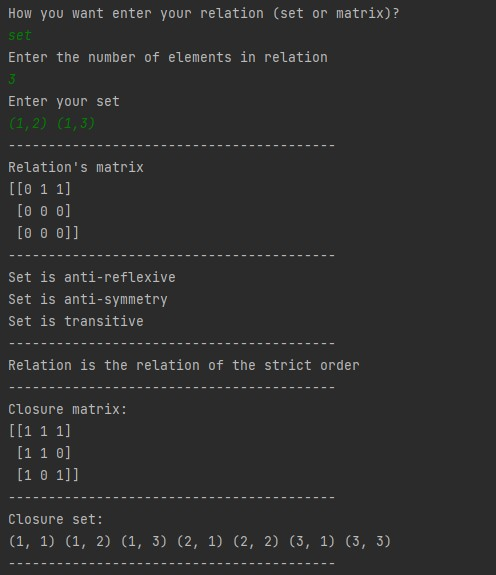
\includegraphics[width=1.\textwidth]{1}
            \caption{Ввод бинарного отношения {(1, 2), (1, 3)} в виде множества с выводом свойств этого множества и замыкания относительно эквивалентности}
            \label{fig:image1}
        \end{figure}

        \subsection{Оценки сложности рассмотренных алгоритмов}

        \subsubsection{Алгоритм определения рефлексивности}

            Сложность выполнения проверки на рефлексивность определяется как $O(n)$.
        
        \subsubsection{Алгоритм определения антирефлексивности}

            За счет схожести с алгоритмом определения рефлексивности сложность определяется как $O(n)$.

        \subsubsection{Алгоритм определения симметричности}

            Cложность транспонирования в numpy определяется как $O(n^{3/2}log \text{ } n)$, сложность сравнение двух матриц поэлементно определяется как $O(n^2)$. 
            Отсюда можно сделать вывод, что сложность алгоритма будет определятся как 
            $O(n^{3/2}log \text{ } n + n^2) = O(n^2)$.

        \subsubsection{Алгоритм определения антисимметричности}

            Сложность поэлементного умножения матриц определяется как $O(n^2)$, сложность сравнение двух матриц поэлементно определяется как $O(n^2)$.
            Отсюда можно сделать вывод, что сложность будет определятся как $O(n^2 + n^2) = O(n^2)$

        \subsubsection{Алгоритм определения транзитивности}

            Из всего выше сказанного очевидно, что сложность проверки на транзитивность или антитранзитивность составляет $O(n^3)$,
            так как в нем используется умножение, сравнение матриц и тройной цикл для проверки рефлексивности в худшем случае матриц.

        \subsubsection{Алгоритм классификации}
            Сложность выполнения самого алгоритма классификации бинарных отношений реализованно через словарь языка python
            и оператор if, поэтому является константной ($O(1)$), если не учитывать сложность выполнения проверки свойств отношения.
            Если учитывать сложность алгоритмов проверки свойств отношения, то :

            \begin{enumerate}
                \item Сложность проверка на квазипорядок определяется как $O(n^3 + n) = O(n^3)$.
                \item Сложность проверка на эквивалентность определяется как $O(n^3 + n + n^{3/2}log \text{ } n) = O(n^3)$.
                \item Сложность проверка на частичный порядок определяется как $O(n^3 + n + n^3) = O(n^3)$.
                \item Сложность проверка на строгий порядок определяется как $O(n^3 + n + n^3) = O(n^3)$.
            \end{enumerate}

        \subsubsection{Построение замыкания рефлексивности}
        
            Так как весь алгоритм строится на заполнении главной диагонали матрицы 1, то его сложность состовляет $O(n)$.

        \subsubsection{Построение замыкания симметричности}

            Для посторения замыкания симметричности используются вложенный цикла, поэтому сложность алгоритма
            определяется как $O(n^2)$.

        \subsubsection{Построение замыкания транзитивности}

            Для посторения замыкания транзитивности используются три вложенный цикла, поэтому сложность алгоритма
            определяется как $O(n^4)$.
    
\conclusion

В рамках данной лабораторной работы были рассмотренны теоритические основы свойств бинарных отношений, их видов и методов
их замыкания по каждому из свойств. На основе этой теоретической части была смоделирована программа на языке Python с 
использованием средств библиотеки Numpy, которая способна определить свойства заданного множества, его вид и построить 
систему замыкания по каждому из основных свойств бинарного отношения, а так же была оценена асимптотика каждого реализованного
алгоритма.

\end{document}
